
%(BEGIN_QUESTION)
% Copyright 2010, Tony R. Kuphaldt, released under the Creative Commons Attribution License (v 1.0)
% This means you may do almost anything with this work of mine, so long as you give me proper credit

This is a PFD for a simple geothermal power plant, drawing a mixture of superheated steam and entrained minerals from a ``production well'' drilled deep into the earth, and injecting the condensed water and minerals into a second ``injection well'' to be re-heated by geothermal heat:

$$\includegraphics[width=15.5cm]{i00070x01.eps}$$

One day an operator notices something strange on the trend graph for the HP separator: the brine level in that separator seems to oscillate in a square-wave manner around the usual setpoint value, but stabilizes at any other setpoint value:

$$\includegraphics[width=15.5cm]{i00070x02.eps}$$

Identify a realistic cause for this strange level-control behavior, and then identify the next step you would take to diagnose and rectify the problem.

\vfil

\underbar{file i00070}
\eject
%(END_QUESTION)





%(BEGIN_ANSWER)

This is a graded question -- no answers or hints given!

%(END_ANSWER)





%(BEGIN_NOTES)

If might be tempting to declare this control loop is acting too aggressively, based on the oscillation around setpoint that we see at the beginning of the trend.  However, note that the loop does not oscillate around setpoint near the end of the trend, which is unusual if the problem is simply too much gain (or other controller action).  No, the problem here is more complex than this.

\vskip 10pt

It might also be tempting to declare that the HP separator control valve is sticky, given the flat-line response of the PV from time to time.  This, however, is not how a liquid level control loop will typically react with a sticky valve.  When the valve sticks in a liquid level control loop, the level will either ramp down or ramp up (unless the valve just happens to stick at precisely the ``balance'' point of the process!).  T

\vskip 10pt

The clue to determining the source of the problem here is how the PV trend ``sticks'' (exhibits {\it flat} periods) and the {\it suddenly} jumps to new values, much faster than the process level is actually capable of changing as indicated by the other rises and falls of the PV.  This indicates the level transmitter itself is alternately {\it non-responsive} to regular fluctuations in brine level.  The control system sees a non-responding level away from setpoint and acts to bring it back toward setpoint.  If the level goes beyond setpoint and then the transmitter ``unsticks'' to measure the new level, the wind-up cycle repeats.

\vskip 10pt

A good ``next step'' to take would be to remove the transmitter from service and ``stimulate'' it throughout its full range of level measurement to see if you can reproduce the ``sticking'' behavior seen here.

\vskip 10pt

If this is a displacer-type instrument, accumulations of salts around the displacer (inside the cage) could account for this behavior.  As soon as the level gets away from the normal setpoint value, the transmitter responds normally and all is well.

%INDEX% Process troubleshooting: diagnosing problem via trend recording
%INDEX% Process: geothermal power plant

%(END_NOTES)


